\begin{figure}[ht]
\centering
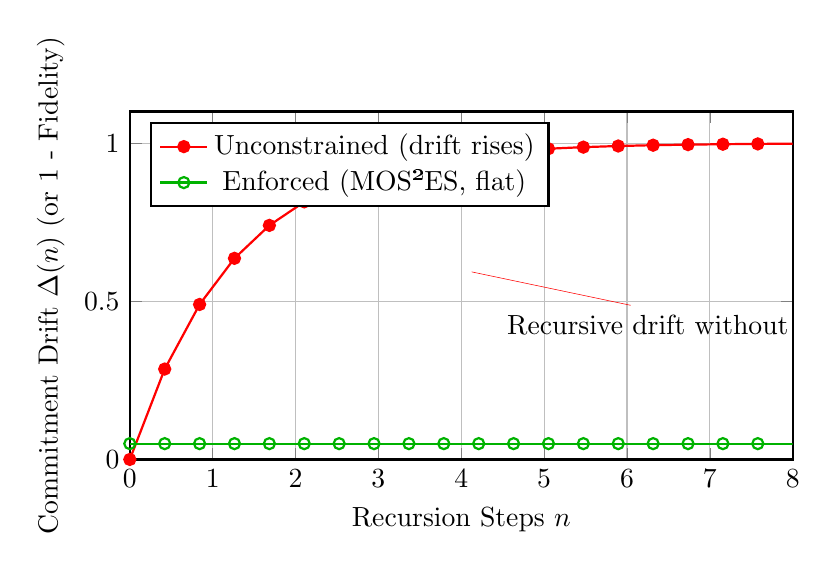
\begin{tikzpicture}
\begin{axis}[
    width=10cm, height=6cm,
    xlabel={Recursion Steps $n$},
    ylabel={Commitment Drift $\Delta(n)$ (or 1 - Fidelity)},
    xmin=0, xmax=8,
    ymin=0, ymax=1.1,
    grid=major,
    legend pos=north west,
    thick
]

% Unconstrained: exponential-like drift
\addplot[red, mark=*, domain=0:8, samples=20] {1 - exp(-0.8*x)}; 
\addlegendentry{Unconstrained (drift rises)}

% Enforced: flat near 0
\addplot[green!70!black, mark=o, domain=0:8, samples=20] {0.05}; 
\addlegendentry{Enforced (MOS²ES, flat)}

\node at (axis cs:4,0.6) [pin={[pin edge={red}]-45:{Recursive drift without enforcement}}] {};

\end{axis}
\end{tikzpicture}
\caption{Commitment drift (or inverted fidelity) vs. recursion cycles. Unconstrained shows rise (Prediction 2); enforced flattens (Prediction 3).}
\label{fig:drift-recursion}
\end{figure}